% The names of the semi-Lagrangian point schemes, as a UML class diagram.
% A scheme name is OWN-NEIGHBOUR/SPACE+TRANSITION. Each of the four parts is one
% family of alternatives. The executable definition is sympy/scheme_matrix.py.
% Build: make scheme-names-figure   (needs tikz-uml.sty, see the Makefile target)
\documentclass[border=4pt]{standalone}
\usepackage[T1]{fontenc}
\usepackage{lmodern}
\usepackage{tikz-uml}
\newcommand{\tok}[1]{\texttt{\bfseries #1}}
\begin{document}
\sffamily
\begin{tikzpicture}
\tikzumlset{fill class=white, font=\sffamily}
\umlclass[x=10.05, y=0]{Scheme}{
  name = \tok{OWN-NEIGHBOUR/SPACE+TRANSITION}\\
  \tok{C-Cp/L2}\quad the original scheme\\
  \tok{BFC/I+c}\quad tensor set in 2D, hanging points constrained\\
  \tok{C-Cp/L2+g}\quad the original scheme with ghost cells}{
  step: every unknown takes the value of the\\ reconstruction $R$ at its departure point}
\umlclass[x=0.00, y=-4.60, type=abstract, width=4.4cm]{OWN}{}{the points of a cell that\\ carry advected unknowns}
\umlclass[x=2.10, y=-7.90, width=4.7cm]{C}{cell centre}{unknowns per cell:\\ 1 (3D), 1 (2D)}
\umlclass[x=2.10, y=-10.96, width=4.7cm]{SC}{simple cubic:\\ vertices}{unknowns per cell: 1, 1}
\umlclass[x=2.10, y=-14.03, width=4.7cm]{BCC}{body-centred cubic:\\ centre + vertices}{unknowns per cell: 2, 2}
\umlclass[x=2.10, y=-17.09, width=4.7cm]{FCC}{face-centred cubic:\\ vertices + face centres}{unknowns per cell: 4, 3}
\umlclass[x=2.10, y=-20.38, width=4.7cm]{BFC}{body- and face-centred:\\ centre + vertices\\ + face centres}{unknowns per cell: 5, 4}
\umlclass[x=2.10, y=-24.15, width=4.7cm]{T}{tensor: centre + vertices\\ + face centres\\ + edge midpoints}{unknowns per cell: 8 (3D);\\ in 2D equal to \tok{BFC}}
\foreach \c in {C, SC, BCC, FCC, BFC, T} {\umlinherit[geometry=-|, anchor1=180, anchor2=-125]{\c}{OWN}}
\umlclass[x=6.70, y=-4.60, type=abstract, width=4.4cm]{NEIGHBOUR}{}{cell-centre values read\\ from neighbour cells}
\umlclass[x=8.80, y=-7.69, width=4.7cm]{no neighbour}{no suffix:\\ own points only}{}
\umlclass[x=8.80, y=-11.02, width=4.7cm]{-Cf}{centres of the face\\ neighbours (OpenFOAM\\ cell-face-cell)}{cells: 6 (3D), 4 (2D);\\ needs a centre in OWN}
\umlclass[x=8.80, y=-15.02, width=4.7cm]{-Cp}{centres of the point\\ neighbours (OpenFOAM\\ cell-point-cell)}{cells: 26 (3D), 8 (2D);\\ needs a centre in OWN}
\foreach \c in {no neighbour, -Cf, -Cp} {\umlinherit[geometry=-|, anchor1=180, anchor2=-125]{\c}{NEIGHBOUR}}
\umlclass[x=13.40, y=-4.60, type=abstract, width=4.4cm]{SPACE}{}{the polynomial that is read\\ at the departure point}
\umlclass[x=15.50, y=-7.93, width=4.7cm]{/I}{interpolating: the\\ lowest-degree space that\\ returns every datum exactly}{}
\umlclass[x=15.50, y=-11.27, width=4.7cm]{/L2}{least squares: complete\\ quadratic, weights 1/distance\\ to the cell centre, anchored\\ on the centre value}{}
\foreach \c in {/I, /L2} {\umlinherit[geometry=-|, anchor1=180, anchor2=-125]{\c}{SPACE}}
\umlclass[x=20.10, y=-4.60, type=abstract, width=4.4cm]{TRANSITION}{}{the treatment of a 2:1\\ refinement transition}
\umlclass[x=22.20, y=-7.69, width=4.7cm]{free}{no suffix: a hanging point\\ is an independent unknown}{}
\umlclass[x=22.20, y=-11.25, width=4.7cm]{+c}{constrained: a hanging\\ point carries no unknown;\\ its value is the interpolant\\ of the cell it hangs on}{needs point unknowns\\ (OWN is not \tok{C})}
\umlclass[x=22.20, y=-15.72, width=4.7cm]{+g}{ghost cells: every cell reads\\ a uniform stencil at its own\\ size. Restriction: mean of\\ the fine values. Prolongation:\\ the coarse cell's reconstruction}{needs OWN = \tok{C}}
\foreach \c in {free, +c, +g} {\umlinherit[geometry=-|, anchor1=180, anchor2=-125]{\c}{TRANSITION}}
\umlcompo[geometry=|-|, mult2=1, pos2=2.75]{Scheme}{OWN}
\umlcompo[geometry=|-|, mult2=0..1, pos2=2.75]{Scheme}{NEIGHBOUR}
\umlcompo[geometry=|-|, mult2=1, pos2=2.75]{Scheme}{SPACE}
\umlcompo[geometry=|-|, mult2=0..1, pos2=2.75]{Scheme}{TRANSITION}
\end{tikzpicture}
\end{document}
